\documentclass{article}
\pagestyle{empty}

% \usepackage{soul}
% \usepackage{url}
% \usepackage[hidelinks]{hyperref}
% \usepackage[utf8]{inputenc}
% \usepackage[small]{caption}
% \usepackage{graphicx}
% \usepackage{amsmath}
% \usepackage{amsthm}
% \usepackage{booktabs}
% \usepackage{algorithm}
% \usepackage{algorithmic}
% \usepackage[switch]{lineno}
\usepackage{xspace}
% % Include other packages here, before hyperref.
\usepackage{svg}


% Support for easy cross-referencing
% \usepackage[capitalize]{cleveref}
% \crefname{section}{Sec.}{Secs.}
% \Crefname{section}{Section}{Sections}
% \Crefname{table}{Table}{Tables}
% \crefname{table}{Tab.}{Tabs.}

% \usepackage[normalem]{ulem}
\usepackage{amsmath}
\usepackage{amssymb}
\usepackage[inline]{enumitem}
\usepackage{caption}
\usepackage{subcaption}
\usepackage{makecell}
\usepackage{tikz}
\usepackage{pgfplots}
\usepackage{booktabs}
\newcommand{\ours}[0]{ElasticViT\xspace}
\newcommand{\dmodel}{d_{\text{model}}}
\newcommand{\afterplot}{} %\vspace{-.15in}}
\usepackage{amsthm}
\newtheorem{observation}{Observation}
\newtheorem{lemma}{Lemma}


\newcommand{\todo}[1]{\textcolor{red}{[#1]}}
\newcommand{\old}[1]{\textcolor{gray}{[#1]}}

\newcommand{\janek}[2]{\textcolor{red}{#1} \textcolor{blue}{[janek: #2]}}

\DeclareMathOperator{\pred}{pred}
\DeclareMathOperator{\E}{E}
\DeclareMathOperator{\miss}{miss}
\DeclareMathOperator{\scale}{scale}
\DeclareMathOperator{\pos}{pos}
\DeclareMathOperator{\PE}{PE}


\title{Theoretical analysis of input sampling strategies and their impact on positional embedding}

\begin{document}
% \maketitle

\section*{Definition recall}
To strictly define the evaluation pipeline, let us consider image $I$ for which we generate set $P$ of patches $p = (x, y, s)$, where $x$ and $y$ denote the top-left corner's coordinates, and $s$ represents the relative scale (i.e. we sample a patch $r \cdot s \times r \cdot s$ and rescale it bilinearly to size $r \times r$). Initially, the coordinates $x$ and $y$ are from the regular grid and $s=1$. However, in the next step, we perturb them with three functions corresponding to the considered elasticities:
\begin{itemize}
\item $\E_{\scale(s_1, s_2)}(P)$ - introduces the scale perturbations,  sampling the $s$ parameter of every patch $p \in P$ independently and uniformly from range $[s_1, s_2]$.
\item $\E_{\miss(d)}(P)$ - adds missing data perturbations, dropping out $d$ patches from $P$ randomly with equal probability. 
\item $\E_{\pos(q)}(P)$ - applies positional perturbation, modifying $x$ and $y$ parameters of each patch $p \in P$, independently moving them by offsets sampled uniformly from range $[-r \cdot q, r \cdot q]$, where $r$ is the size of the patch.
\end{itemize}

The patches are described by their upper left $(x, y)$ and lower right corner $(x + rs, y+rs)$. Then each coordinate $\pos \in \{x, y, x+rs, y+rs\}$ is encoded by the sinusoidal positional encoding:
\begin{align*}
    \PE_{(\pos,2i)} &= \sin\left(\frac{\pos}{10000^{2i/l}}\right) \\
    \PE_{(\pos,2i+1)} &= \cos\left(\frac{\pos}{10000^{2i/l}}\right).
\end{align*}
which are concatenated into a single vector.

\section*{Perturbations influence on positional embedding}

The application of $\E_{\miss}$ does not affect the positional encoding of a patch. However, if a patch was not dropped by the $\E_{\miss}$ perturbation, then the other two perturbations can modify its position embedding.

After application of $\E_{\pos}$, the values of $x$ and $y$ get updated to $x+ \Delta x$, $y+\Delta y$, while the lower right corner $x+rs$ and $y+rs$ get updated to values $x + rs + \Delta x$ and $y + rs + \Delta y$. The offset values $\Delta x$ and $\Delta y$ do not depend on $x$ nor $y$. Thus, for $x$, we obtain the following positional embedding
\begin{align*}
    \PE_{(x + \Delta x,2i)} &= \sin\left(\frac{x}{10000^{2i/l}} + \frac{\Delta x}{10000^{2i/l}}\right) \\
    \PE_{(x + \Delta x,2i+1)} &= \cos\left(\frac{x}{10000^{2i/l}} + \frac{\Delta x}{10000^{2i/l}}\right),
\end{align*}
which holds analogously for the other three coordinates $\{y, x+rs, y+rs\}$.

When it comes to $\E_{\scale}$, it modifies the $s$ value to $s + \Delta s$ therefore $\pos \in \{x, y\}$ remains unchanged, while both coordinates $\pos \in \{x + rs, y + rs\}$ are offset by the value $\Delta = r\Delta s$. The formula is analogous to the $\E_{\pos}$ case.

% To obtain further observations we need a technical lemma.
% \begin{lemma}
% The following algebraic equation holds for any $\alpha$ and $\beta$
%     $$(\sin(\alpha + \beta) - \sin(\alpha))^2 + (\cos(\alpha + \beta) - \cos(\alpha))^2 = 4 
%  \sin^4(\alpha / 2) + \sin^2(\beta).$$
% \end{lemma}

% \begin{proof}
%     Recall the trigonometric identities for sum of arguments
%     \begin{align*}
%     \sin(\alpha + \beta) &= \sin(\alpha)\cos(\beta) + \cos(\alpha)\sin(\beta)\\
%     \cos(\alpha + \beta) &= \cos(\alpha)\cos(\beta) - \sin(\alpha)\sin(\beta).
%     \end{align*}
% After applying the above identities to the LHS of the equation we obtain
%  $$(\sin(\alpha)(\cos(\beta) - 1) + \cos(\alpha)\sin(\beta))^2 + (\cos(\alpha)(\cos(\beta)-1) - \sin(\alpha)\sin(\beta))^2.$$
% After squaring, grouping the terms and applying $\sin^2 + \cos^2 = 1$ we get
% $$
% (\cos(\alpha)-1)^2 + \sin^2(\beta).
% $$
% Note that $(\cos(\alpha)-1)^2 = 4\sin^4(\alpha/2)$ hence we get the result.

% \end{proof}

% We analyze the components of $\PE$ for each pair $(2i, 2i+1)$ and $\pos$ individually while $l$ is a chosen constant. Let's denote, $\alpha = \frac{\pos}{10000^{2i/l}}$ and $\beta = \frac{\Delta}{10000^{2i/l}}$. Note that in the setting of our paper $\pos, \Delta \leq 224$ and $2i \in [0, l]$. Therefore for big values of $i$, both $\alpha$ and $\beta$ are near 0, while for $i=0$, the values of $\alpha$ and $\beta$ range multiple periods of $\sin$.

% \begin{observation}
%     The initial value of $\pos$ and the offset value of $\Delta$ induced by perturbations $\E_{\scale}$ and $\E_{\pos}$ influence the deviation of $\left(\PE_{(\pos', 2i)},\PE_{(\pos', 2i+1)}\right)^T$ from $\left(\PE_{(\pos, 2i)},\PE_{(\pos, 2i+1)}\right)^T \in \mathbb{R}^2$ independently.
% \end{observation}
% \begin{proof}
%     Consider squared euclidean distance between $\left(\PE_{(\pos', 2i)},\PE_{(\pos', 2i+1)}\right)^T$ and $\left(\PE_{(\pos, 2i)},\PE_{(\pos, 2i+1)}\right)^T$
    
%     $$
%     \left(\PE_{(\pos', 2i)} - \PE_{(\pos, 2i)}\right)^2 + \left(\PE_{(\pos', 2i+1)} - \PE_{(\pos, 2i+1)}\right)^2.
%     $$
%     Using the introduced definitions of $\alpha$ and $\beta$, the above is equal to
%     $$
%     (\sin(\alpha + \beta) - \sin(\alpha))^2 + (\cos(\alpha + \beta) - \cos(\alpha))^2.
%     $$
%     By Lemma 1. we obtain
%     $$\left(\PE_{(\pos', 2i)} - \PE_{(\pos, 2i)}\right)^2 + \left(\PE_{(\pos', 2i+1)} - \PE_{(\pos, 2i+1)}\right)^2 = 4\sin^4(\alpha / 2) + \sin^2(\beta).$$
% \end{proof}

% As a direct consequence of the above proof we get another observation.
% \begin{observation}
%     For big values of $i$, when the values of $\alpha$ and $\beta$ are small, the component $\Delta$ is the most significant deviation factor of $\PE_{\pos'}$ from $\PE_{\pos}$.
% \end{observation}
% \begin{proof}
%     Using Taylor's expansion
%     $\sin(\theta) = \theta + o(\theta^2)$ we obtain
%     \begin{align*}
%     4\sin^4(\alpha/2) &= \frac{1}{4} \alpha^4 + o(\alpha^5)\\
%     \sin^2(\beta) &= \beta^2 + o(\beta^3).
%     \end{align*}
%     Now consider the derivatives 
%     \begin{align*}
%     \frac{d}{d\alpha} \left(4\sin^4(\alpha / 2) + \sin^2(\beta) \right) &= \alpha^3 + o(\alpha^4)\\
%     \frac{d}{d\beta} \left(4\sin^4(\alpha / 2) + \sin^2(\beta) \right) &= 2\beta + o(\beta^2).
%     \end{align*}
%     For $\alpha$ and $\beta$ close enough to $0$, $\alpha^3 << 2\beta$. Hence $\Delta$ is the most significant component driving the deviation change.
% \end{proof}

% The above observation in the context of $\E_{\scale}$ can be interpreted that while earlier components depend on both $\pos$ and $s$, the later components of $\PE$ vector are mostly dependent on scale $s$.

\pagebreak

% \section*{Patch sampling strategies cont.}

% \subsection*{Active visual exploration}

% \begin{table}[t]
\caption{\textbf{Active visual exploration results:} We evaluate the performance of ElasticViT with MAE-like decoder head compared to standard MAE in active visual exploration scene reconstruction task performed by the AME algorithm. The metric is root mean squared error (RMSE; lower is better) and the dataset is ImageNet-1k. Our method outperforms competitive solutions.}
\label{tab:ame}
\begin{center}
\begin{small}
\vspace{-.2cm}
\begin{tabular}{l@{\hskip20pt}l}
\toprule
Method & RMSE \\
\midrule
MAE + AME & 30.5  \\
\textbf{ElasticMAE + AME (dual resolution)} & 25.95 \\
\textbf{ElasticMAE + AME (quad tree)} & \textbf{23.2}  \\
\bottomrule
\end{tabular}
\end{small}
\end{center}
\end{table}

% To asses the performance of our method on practical task, which benefit from elastic sampling we apply it to active visual exploration. For this experiment, we use the AME exploration algorithm~\cite{pardyl2023active}, replacing the ViT encoder of the backbone MAE model with our ElasticViT. We pre-train resultant encoder-decoder architecture (ElasticMAE) on ImageNet-1k with standard ElasticViT training regime and then fine-tune the entire exploration model using the original AME training code. The image resolution is $224\times224$ and the exploration process at each of $12$ steps samples a square fragment (glimpse) consisting of $2\times2$ patches.

% As AME uses only single scale sampling, we consider two simple modifications for it to support variable scale exploration: \begin{itemize}
%     \item dual resolution AME - we start with a low-resolution glimpse covering the entire image (scale = $3.5$) and follow with 11 high resolution glimpses (scale = 1).
%     \item quad tree AME - as above we start with a low-resolution glimpse (scale = 3.5), then at each step we use AME to select a patch which is the best candidate for exploration and perform the next glimpse at its location. Effectively at each step we divide one existing patch into four new ones of higher resolution.
% \end{itemize}.

% Regardless of the glimpse regime, as the native patch size is $16\times16$, all methods use 25\% of the scene resolution. ElasticViT backed AME outperforms the baseline with a significant margin, see Tab.~\ref{tab:ame}.


\begin{figure}[t]
\begin{center}
\begin{small}
\begin{sc}
\begin{center}
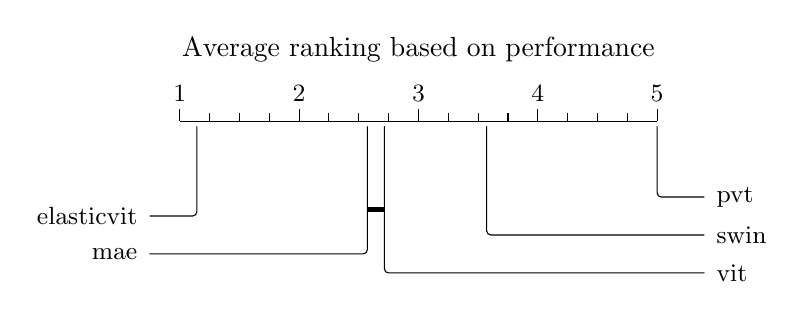
\begin{tikzpicture}[
  treatment line/.style={rounded corners=1.5pt, line cap=round, shorten >=1pt},
  treatment label/.style={font=\small},
  group line/.style={ultra thick},
]

\begin{axis}[
  clip={false},
  axis x line={center},
  axis y line={none},
  axis line style={-},
  xmin={1},
  ymax={0},
  scale only axis={true},
  width={.5\linewidth},
  ticklabel style={anchor=south, yshift=1.3*\pgfkeysvalueof{/pgfplots/major tick length}, font=\small},
  every tick/.style={draw=black},
  major tick style={yshift=.5*\pgfkeysvalueof{/pgfplots/major tick length}},
  minor tick style={yshift=.5*\pgfkeysvalueof{/pgfplots/minor tick length}},
  title style={yshift=\baselineskip},
  xmax={5},
  ymin={-3.5},
  height={4\baselineskip},
  xtick={1,2,3,4,5},
  minor x tick num={3},
  title={Average ranking based on performance},
]

\draw[treatment line] ([yshift=-2pt] axis cs:1.1428571428571428, 0) |- (axis cs:0.726190476190476, -2.5)
  node[treatment label, anchor=east] {elasticvit};
\draw[treatment line] ([yshift=-2pt] axis cs:2.5714285714285716, 0) |- (axis cs:0.726190476190476, -3.5)
  node[treatment label, anchor=east] {mae};
\draw[treatment line] ([yshift=-2pt] axis cs:2.7142857142857144, 0) |- (axis cs:5.416666666666667, -4.0)
  node[treatment label, anchor=west] {vit};
\draw[treatment line] ([yshift=-2pt] axis cs:3.5714285714285716, 0) |- (axis cs:5.416666666666667, -3.0)
  node[treatment label, anchor=west] {swin};
\draw[treatment line] ([yshift=-2pt] axis cs:5.0, 0) |- (axis cs:5.416666666666667, -2.0)
  node[treatment label, anchor=west] {pvt};
\draw[group line] (axis cs:2.5714285714285716, -2.3333333333333335) -- (axis cs:2.7142857142857144, -2.3333333333333335);

\end{axis}
\end{tikzpicture}
\end{center}
\end{sc}
\end{small}
\end{center}
\afterplot
\caption{\textbf{Critical difference diagram}: Average performance ranking of \ours{} and baseline methods for ImageNet with high perturbation (most extreme settings). \ours{} significantly outperforms remaining approaches, while more structured methods (PVT and Swin) perform significantly worse than simple ViT. Moreover, the difference between ViT and MAE is insignificant. Notice that this diagram was generated for rankings generated based on results from Fig.~4 and Fig.~5 of the main paper. %~\ref{fig:zoom-sample}, \ref{fig:dropout-sample}, \ref{fig:shake-sample}, and \ref{fig:mixes}.
}
\label{fig:critdist}
\end{figure}


\pagebreak
%\section*{Qualitative results of different sampling perturbations}

\begin{figure}
    \makebox[\textwidth][c]{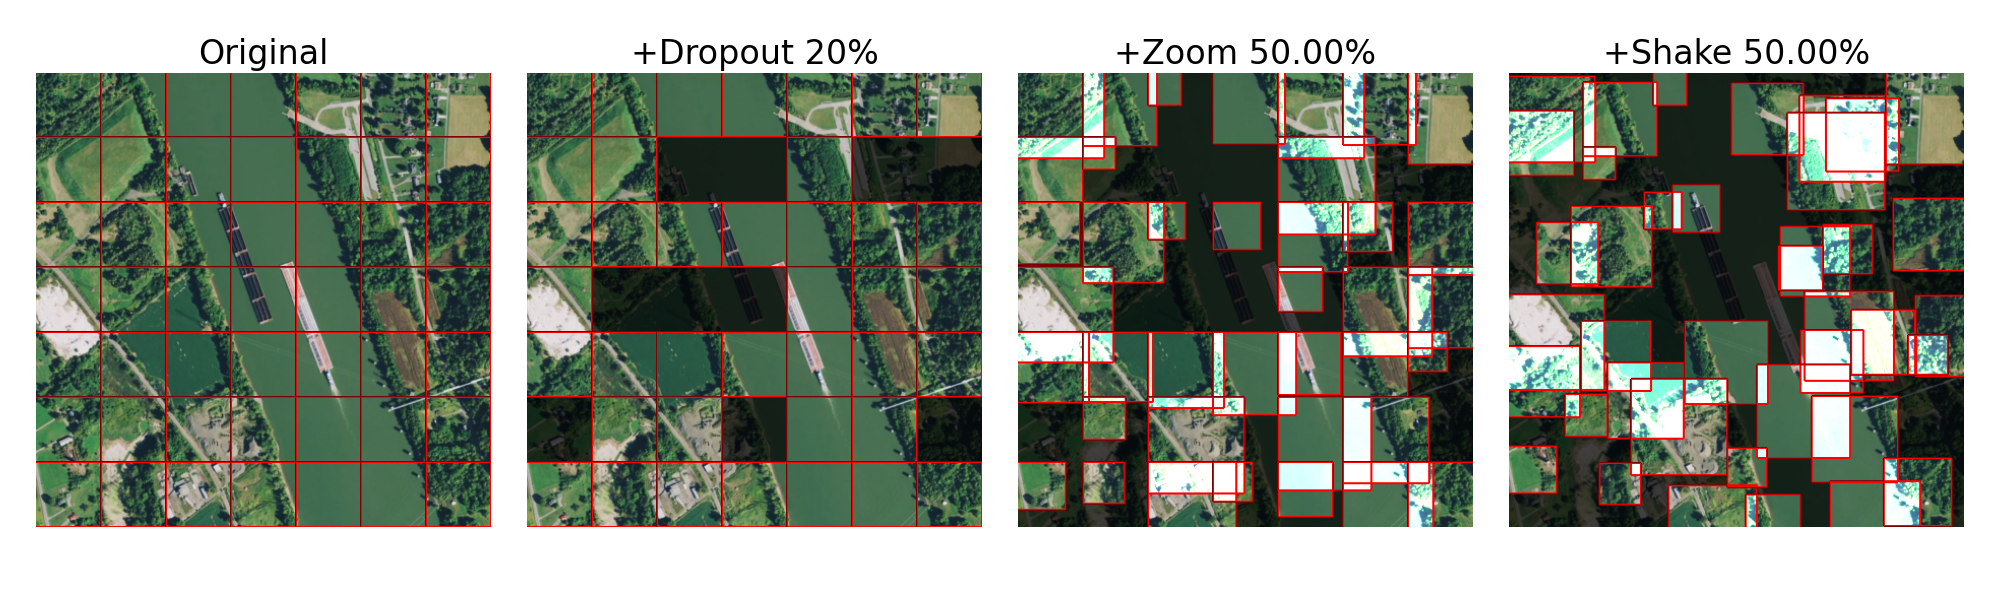
\includegraphics[width=1.3\textwidth]{imgs/aerial_example_10_32_32.png}} \\ 
    \makebox[\textwidth][c]{
\includegraphics[width=1.3\textwidth]{imgs/imgs_448_64/config_10_32_32/img_1.png}} \\
    \makebox[\textwidth][c]{
\includegraphics[width=1.3\textwidth]{imgs/imgs_448_64/config_10_32_32/img_2.png}} \\ 
    \caption{\textbf{Elasticity pipeline visualization:} In this figure, we present visualizations of successive input data perturbations. For clarity, patch borders are marked in red, and patch overlap is highlighted.}
    \label{fig:elasticity-vis}
\end{figure}


\pagebreak

\begin{figure}[t]
    \centering
    \includegraphics[scale=0.7]{figures/hist.pdf}
    \caption{\textbf{Elastic sampling impact on performance across multiple runs:} The histogram represents the distribution of classification error for five inference runs with different random seeds used for elastic sampling. We observe that the differences between runs are insignificant. Note that the accuracy scores of particular runs are provided in the plot legend.}
    \label{fig:seedcheck}
\end{figure}

\end{document}


